%
The given equation can be expressed as 
\begin{align} \label{5/12/Eq b}
\myvec{5 & -7}\vec{x} =9 
\end{align}
Let 
\begin{align}
\vec{x}=\myvec{a\\0}
\end{align}
Substituting in  \eqref{5/12/Eq b},
\begin{align}
\myvec{5 & -7} \myvec{a\\0} &= 9
\\
\implies a & = \frac{9}{5}
\end{align}
Similarly,
\begin{align}
\vec{x}=\myvec{0\\b}
\end{align}
Substituting in  \eqref{5/12/Eq b},
\begin{align}
\myvec{5 & -7} \myvec{0\\b} &= 9
\\ \implies b &= \frac{-9}{7}
\end{align}
So, the intercepts of X and Y axes can be obtained as,
\begin{align}
\vec{A}=\myvec{\dfrac{9}{5}\\0} , 
\vec{B}=\myvec{0\\\dfrac{-9}{7}}
\end{align}
%
See Fig. \ref{5/12/fig}.
%
\begin{figure}[!ht]
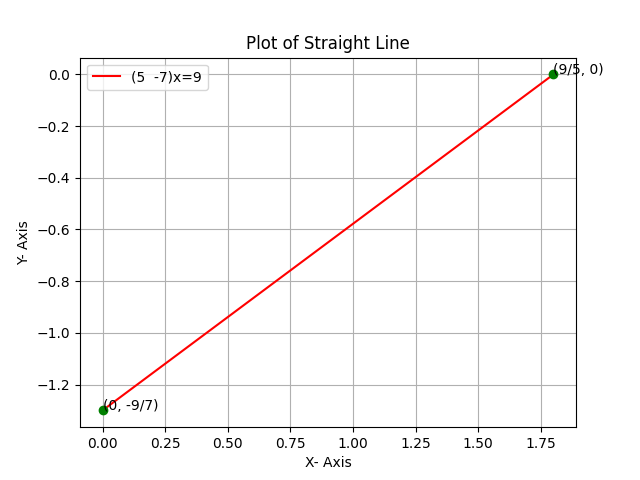
\includegraphics[width=\columnwidth]{Figure_1.png}
\caption{ Plot of the straight line }
\label{5/12/fig}
\end{figure}












